
%%%%%%%%%%%%%%%%%%%%%%%%%%%%%%%%%%%%%%%%%%%%%%%%%%%%%%%%%%%%%%%%%%%%%%%%
\chapter{Probability and Statistics Analysis} \label{sec_probsnstat}
%%%%%%%%%%%%%%%%%%%%%%%%%%%%%%%%%%%%%%%%%%%%%%%%%%%%%%%%%%%%%%%%%%%%%%%%

% QUESTION: SHOULD I SPECIFY THAT FB IS RE 1 MICROPA2/HZ

%%%%%%%%%%%%%%%%%%%%%%%%%%%%%%%%%%%%%%%%%%%%%%%%%%%%%%%%%%%%%%%%%%%%%%%%
\section{Introduction to Probability and Statistics Analysis} \label{sec_statintro}
%%%%%%%%%%%%%%%%%%%%%%%%%%%%%%%%%%%%%%%%%%%%%%%%%%%%%%%%%%%%%%%%%%%%%%%% this may not be the best name?

% note to self: stats and probs discussion is very independent of sources/whys, think of this as presenting numbers only

As introduced in \autoref{intro_env_info}, ambient noise in the Arctic can be partitioned into three environmental conditions: 'ice with duct', 'ice without duct', and 'no ice.' Each of these acoustic environments has a unique makeup of ambient noise produced by a variety of drivers and are affected by the factors of the environment. By looking at a broadband range of frequencies, information is gained of how ambient sound operates under each environment and the differences between them.  

A broadband analysis of the ambient noise level (ANL) recorded by the SHRU(s) was performed using the data from SHRU5. To keep consistency with the preliminary study, \parencite{Bonnel2021}, the data for this analysis came from SHRU5, as it had the least self noise compared to other SHRU(s). ANL(s) were computed for a total of 39 frequency bands 50 Hz wide and centered on frequencies 50 Hz apart, from 50 to 1900 Hz. The ANL data was divided into the three acoustic environments for analysis. When comparing sound level values, the units used are dB referenced to $1 \mu Pa/Hz $, later just referred to as dB. % be sure to CLEARLY define these in section before

Though each frequency has some independent qualities, they appear to be quantitatively linked when analyzed using a variety of different statistics. These statistic quantities ranged from single metrics to comparing sound distributions of the entire acoustic environment. While the preliminary study \parencite{Bonnel2021} examined a frequency band around 300 Hz of 250-350 Hz, it can be assumed that this was not the only acoustic frequency propagating through the water. As this analysis would suggest, the frequency range of ambient noise under ice is broad in nature, likely influenced by environmental drivers such as shifting ice \parencite{kinda2015arctic}. This discussion will primarily focus on the numerical quantities and probabilities of ambient noise collected during the duration of CANAPE, independent of time and sources.



%%%%%%%%%%%%%%%%%%%%%%%%%%%%%%%%%%%%%%%%%%%%%%%%%%%%%%%%%%%%%%%%%%%%%%%%
\section{Probability and Statistical Analysis Methods and Results}
%%%%%%%%%%%%%%%%%%%%%%%%%%%%%%%%%%%%%%%%%%%%%%%%%%%%%%%%%%%%%%%%%%%%%%%%

%%%%%%%%%%%%%%%%%%%%%%%%%%%%%%%%%%%%%%%%%%%%%%%%%%%%%%%%%%%%%%%%%%%%%%%%
\subsection{Correlation Between Frequencies} \label{sec_corr_freq}
%%%%%%%%%%%%%%%%%%%%%%%%%%%%%%%%%%%%%%%%%%%%%%%%%%%%%%%%%%%%%%%%%%%%%%%%

Exploring the relationships between frequencies in probability shows these environmental conditions share a significant amount of ambient noise distribution. In \autoref{fig_freq_corr} the correlation between each of the ambient noise levels of each frequency is shown for each of the three environmental conditions. The correlation values range from 0.4758 for 'ice without duct' condition to 1. 

Other than the very lowest frequencies, correlation between almost all of the frequency bands is quite high, $>0.8$.  Each environmental condition does act differently when high and low frequencies are compared to each other, resulting in different correlation graph shapes. 'No ice' has the largest area of high correlation values of the three environments, followed by 'ice with duct', then 'ice without duct.' 'No ice' has bands of lower correlation around 0.8 for the 100-300 Hz comparisons; elsewhere it is approximately 1.

% not entirely sure if i am able to speculate as to why this is, this is just how it is
'No ice' has a boxy bloc of >0.9 correlation while 'ice with duct' and 'ice without duct' have smoother gradients. When high and low frequencies are compared, correlation values are lower (0.8). The correlations for 'ice' conditions seems to be affected more by frequency. 'Ice without duct' has the least amount of high correlation of \autoref{fig_freq_corr}, and the lowest of the three while still showing that most ANL frequencies are very related.

The noise levels definitely share many attributes across all frequencies except 50 Hz. The presence of ice reduces the strength of correlation, and more is lost when the Duct is present. Decreases in correlation could come from the different drivers of ambient noise for these conditions, or the interference of the ice sheet and Duct. \autoref{fig_freq_corr} definitively shows that many frequencies are closely related, but the exact nature of their relationship is not yet shown. This will be explored in the following sections using various statistic metrics. 

%Correlation for 'ice with duct' has the same distinct bands of low correlation at low frequency as the other two graphs, but does not have as distinct of a green band corresponding to 0.7. 'Ice with duct' has a narrower band of high correlation than 'ice with duct' and the middle amount of high correlation values. From about 50 Hz to 1900 Hz correlation values are around 0.9, but once frequencies above 1000 are compared to frequencies below 1000 Hz, correlation drops to around 0.8. 

\begin{figure}[ht]
\centering
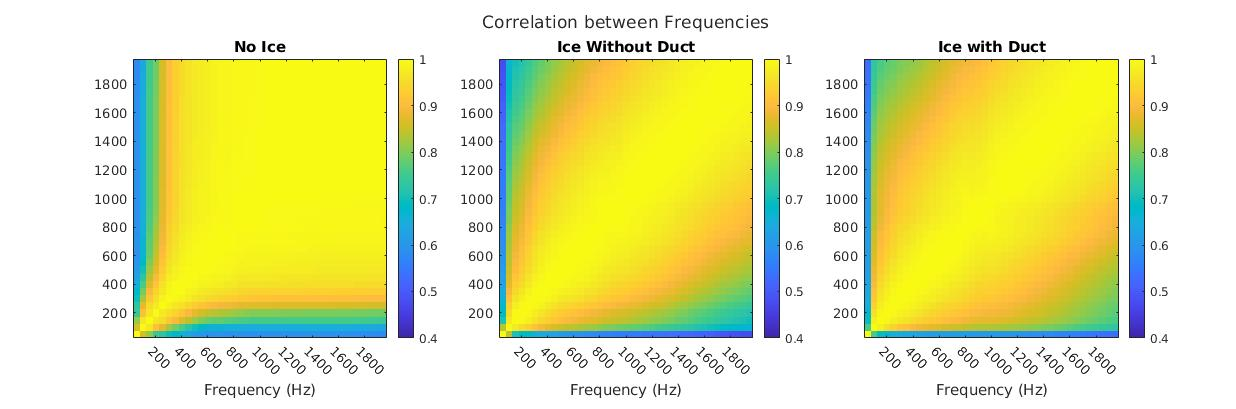
\includegraphics[scale=0.35]{Figures/corr_all_1x3.jpg}
\caption{Correlation between broadband frequencies for 50-1900 Hz}
\label{fig_freq_corr}
\end{figure}

%%%%%%%%%%%%%%%%%%%%%%%%%%%%%%%%%%%%%%%%%%%%%%%%%%%%%%%%%%%%%%%%%%%%%%%%%%%%%%%%%%%%%%%%%%%%%
\subsection{ANL Time Series}\label{sec_timeseries}

From \autoref{sec_corr_freq} it is certain that the ambient noise of most frequencies are highly related, but the complexities of the relationship between frequencies aren't known. Plotting the time series for levels of ambient noise for three selected frequencies in \autoref{fig_timeseries} illustrates how ambient sound operates in time through 500 Hz (blue), 1000 Hz (orange), and 1500 Hz (yellow) for the selected time period of July 2, 2017 to July 9, 2017. %change date as needed

When looking at \autoref{fig_timeseries}, it is obvious that the ambient noise of these three frequencies vary in very similar ways. The oscillation of ANL in time between the three is very synchronous, with peaks and drops happening at almost the same time which explains the high correlation. Where the graphs differ is in the amplitude of the three lines; in general, 500 Hz in blue is usually above 1000 Hz in orange which in turn is above 1500 Hz in yellow. Sound levels through the duration of CANAPE derive from a variety of sources, but the stacking of the ambient noise is consistent in time if observing the entire period over which data was collected. The difference in amplitude remains mostly consistent as well through these frequencies, indicating that ANL tends to decrease while frequency increases. 

Based on \autoref{fig_timeseries}, sound level varies highly but the variations are matched throughout frequencies, with a few exceptions. On July 5,  2017 when all three lines are at the same level, significant events closer to the hydrophone array caused noise levels to be even from 500 to 1500 Hz. Events like these suggest not all of the ambient sound recorded was driven by distant sources; nor is the stratification between frequencies total. Spikes in noise may coincide with significant ice movements, storms, or winds but whatever the driving force of the ambient noise is, it affects all frequencies in a similar way. Knowing that the time series of distant frequencies are related but different in time, the next step is to look at the distribution of levels of ambient noise divided into the environmental conditions of 'ice with duct', 'ice without duct', 'and 'no ice' to observe the effects of the Beaufort Duct.

% note to self. make a figure super zoomed in figure of like one day and unlock the ticks, add units to SPL ANL

\begin{figure}[ht]
\centering
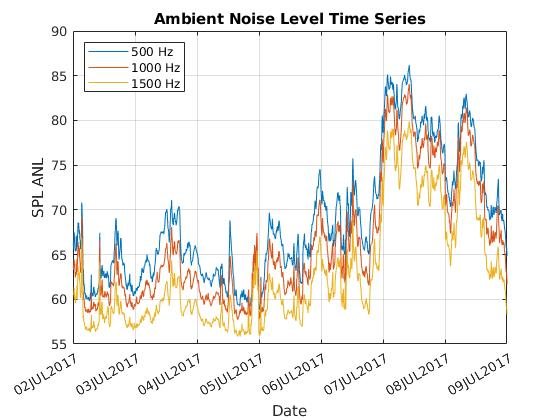
\includegraphics[scale=0.6]{Figures/timeseries_500_1500_july_overlay.jpg}
\caption{Ambient Noise Time series from 02JUL2017 to 09JUL2017 FOR 500 Hz, 1000 Hz, and 1500 Hz showing similar oscillations of ANL}
\label{fig_timeseries}
\end{figure}





%%%%%%%%%%%%%%%%%%%%%%%%%%%%%%%%%%%%%%%%%%%%%%%%%%%%%%%%%%%%%%%%%%%%%%%%%%%%%%%%%%%%%%%%%%%%%
\subsection{The Ambient Noise Histogram} \label{sec_hist}

One of the simplest ways to visualize the differences of ANL under the three environmental conditions is by partitioning the power spectral density (PSD) of ANL in dB into histograms. After computing the ANL(s), the bin size for each histogram was vector of 50 values, ranging from the minimum ANL to the maximum ANL of the frequency through all environmental conditions. The average bin size was around 1 Hz, with the highest frequencies having a slightly smaller bin size (\textasciitilde 0.97) due to their more limited range. % julien note here?

Histograms were normalized using the probability density function (PDF) rather than counts to show the likelihood of this ANL occurring. As the acoustic data is finite, an exact PDF is not possible, leading to an estimate function. The equation for this estimate is

\begin{equation} \label{eq:hist_pdf}
 \nu _{i}=\frac{c_{i}}{N \cdot w_{i}} 
\end{equation}

where $i$ refers to the bin, $\nu _{i}$ is the value of the bin, $c_{i}$ is the number of elements in the bin, and \textit{N} is the number of elements in the input data. The sum of all $\nu_{i}$, the bar size, is equivalent or almost equivalent to 1. Therefore, these histograms give the relative probability  of a specific frequency's ANL under the three acoustic environment conditions. From this, both the range of ambient noise and the most predominant levels are apparent. To demonstrate the conventions of interpreting an ANL histogram, looking at a few significant figures showing the differences in acoustic environment levels is more pragmatic than examining 39 separate figures. (See \autoref{apdx_hist}) Singular metrics summarizing broadband behavior will be described later in sections.

\begin{figure}[h]
\centering
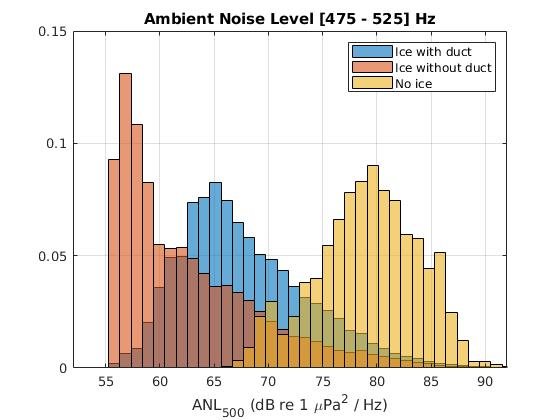
\includegraphics[scale=0.6]{Figures/ANL_500.jpg}
\caption{Histogram of normalized ANL at 500 Hz band for the three major environmental conditions}
\label{fig_hist500}
\end{figure}

%%%%%%%%%%%%%%%%%%%%%%%%%%%%%%%%%%%%%%%%%%%%%%%%%%%%%%%%%%%%%%%%%%%%%%%%%
\subsubsection{Singular Frequency Histogram}
Figure \ref{fig_hist500} is an example of one histogram ranging from 475-525 Hz of the ANL for the three environmental conditions: 'ice with duct',  'ice without duct' and 'no ice'.  The blue histogram is 'ice with duct', the red histogram is 'ice without duct', and the yellow histogram is 'no ice.'  This coloring convention by acoustic environment holds for all statistic figures (\autoref{fig_hist500} to \autoref{fig_peak_prob}) in this section. The number in the bins is less significant than the distribution of the histograms. 

Similar to the earlier study's histogram centered at 300 Hz \parencite{Bonnel2021}, this example (\autoref{fig_hist500}) has three distinct peaks for each unique acoustic environment, displaying a key effect on underwater acoustics from changes to the Arctic environment. The quietest ambient levels occur under 'ice without duct' at 57 dB, then up to 'ice with duct' at 67 dB, and followed by 'no ice' at 80 dB. In terms of shape, the 'no ice' condition histogram qualitatively looks Gaussian in form and = has the shortest range from approximately 65-95 dB. 'Ice with duct' has some right skew and 'ice without duct' is skewed heavily to the right. The two ice conditions have similar ranges from about 62-95 dB, with a matching minimum dB value likely related to the minimum dB measurable by the SHRU(s) at this frequency. This noise floor does change with frequency, as part of the initial setup of the DAQ. \parencite{DAQprocess} %(note that this floor changes with Hz) 

It is commonly said that it is quieter under ice, and \autoref{fig_hist500} directly reflects that through the distribution of ANL in these three different environmental conditions. However, this histogram shows that the presence of the Beaufort Duct increases the levels in the ambient noise distribution at this particular bandwidth of 500 Hz. When the Duct is present, the ANL is likely to be 10 dB higher than an acoustic environment without the Duct. Though the range of the two 'ice' conditions is similar, their distributions are markedly different at least in this specific frequency band. This is further demonstrated in the following sections, where the phenomena usually exists for other frequencies, but not always. %add more explain


\begin{figure}[h]
\centering
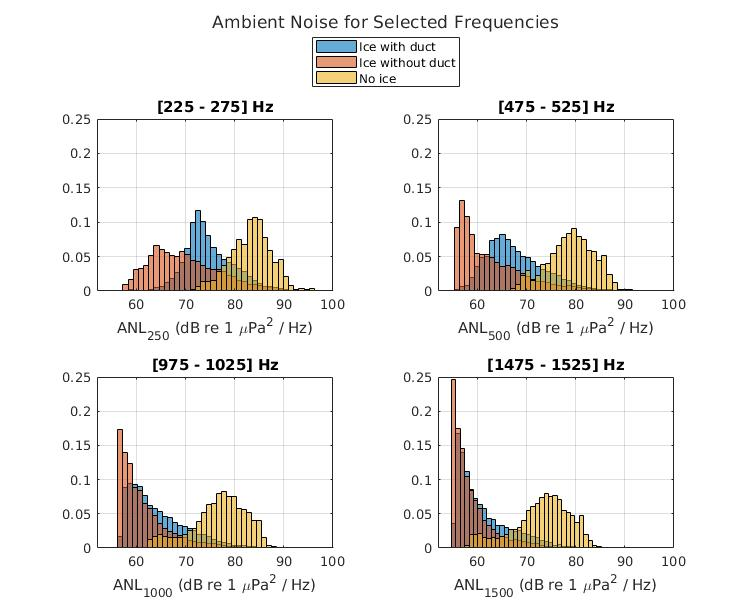
\includegraphics[scale=0.5]{Figures/selected_hists2.jpg}
\caption{Histograms of ANL for 250, 500, 1000, and 1500 Hz}
\label{fig_selhist}
\end{figure}
%\textbf{Shape}

%%%%%%%%%%%%%%%%%%%%%%%%%%%%%%%%%%%%%%%%%%%%%%%%%%%%%%%%%%%%%%%%%%%%%%%%%% order above?
\subsubsection{Multiple Frequencies of Ambient Noise Histograms Compared}
Interpreting one histogram allows its general attributes to be discussed, but more are needed to examine the intricacies of ANL over greater frequency range. In this section, four histograms at frequencies 250, 500, 1000, and 1500 Hz are presented on the same axes in \autoref{fig_selhist}. Note the longitudinal and vertical scales are the same for all histograms for direct comparison, from 55 to 100 dB on the x-axis, and 0 to 0.25 on the y-axis. Both the distribution and shape of these ANL histograms changes as frequency increases. 


One of the most interesting aspects of the \autoref{fig_hist500} above is the sharp difference in layout between 'ice with duct' and 'ice without duct'. This phenomena of three separate peaks is only visible from approximately 100 to 700 Hz. The largest separation between the three bins lies between the frequencies of 150 Hz to 500 Hz. Beyond 700 Hz, the red and blue bars overlap as the sound separation dissipates. This three peak ANL phenomena could be caused by a variety of factors. Perhaps only a small band of certain frequencies travel well through the Duct or are generated into the Beaufort Duct, though none of these reasons are certain.

The range of decibel levels covered by the three environmental conditions decreases as frequency increases. From the upper left panel of \autoref{fig_selhist} at 250 Hz, the ANL decreases from a range of 50 dB to a range of only 35 dB for 1500 Hz. In addition to the diminishing range, there is a general shift down in values for the three environmental conditions. The peak occurrence of 'no ice' ANL(s) decreases 10 dB through frequencies; maximum values of the bars also decrease with frequency. 'No ice' is the loudest of the three conditions for all frequencies; its peak values are usually 10-20 dB more than the others. The other 'ice' environmental conditions do not behave similarly to the 'no ice' trends in ANL distribution. This generalizes the empirical observations of \autoref{fig_selhist}. 

% he 250 Hz histogram for all three conditions has a range of almost 50 db, from approximately 57 to 100 dB. In contrast, the bottom right histograms at 1500 Hz cover a diminished range of 55 to 85 dB. The 35 dB long high frequency range is about 15 dB less than the low frequency range. The intermediate graphs of 500 and 100 Hz reflect this decreasing range of decibel values as the bar distribution becomes tighter.

The red bars for the 'ice without duct' histogram of \autoref{fig_selhist} shift down in peak value while increasing percentage as frequency goes up. When frequency increases for 'ice without duct' the minimum ANL value and maximum bar height tend to align, seen in the 1000 Hz and 1500 Hz graphs. 'Ice without duct' is always the minimum amount of ANL out of all three conditions through all frequencies. 'Ice with duct' is similar to 'ice without duct' at the high frequencies, but differs in the mid to low bands. The red and blue bars align at 1000 and 1500 Hz as the minimum ANL becomes the most predominant noise level. As frequency increases, the maximum bar height also increases for 'ice with duct'.

The shape of the histograms varies highly throughout. For 250 Hz and below all three environmental conditions have a mostly Gaussian shape, but above 250 Hz the shapes diverge. The 'no ice' histogram maintains a mostly normal shape through the whole range of frequencies. Without ice to dampen it, ambient sound is likely driven by air-sea interaction. Toward the highest frequencies, there is some left skew to the 'no ice' histograms, which may be related to the lowered presence of the high frequencies altogether. It does not follow the pattern of the 'ice' environmental condition histograms.

Most of the changes in shape are seen in the red and blue histograms of the ice environment. Above 250 Hz, the 'ice without duct' histogram becomes predominantly right skewed. This right skew emphasizes that the highest occurring noise levels are the lowest values, and that the minimum sound levels occur under 'ice without duct'. 'Ice with duct' is normal in shape up to 350 Hz, then begins skew right. At around 1000 Hz, the histograms for 'ice with duct' and 'ice without duct' are both right skewed and heavily overlapped. The right skew and overall shift down in values reflect the quieter nature of sound under ice and at higher frequency. It is apparent that are high sound levels with ice than without.

% what does it mean



%%%%%%%%%%%%%%%%%%%%%%%%%%%%%%%%%%%%%%%%%%%%%%%%%%%%%%%%%%%%%%%%%%%%%%%%%
\subsection{Average ANL} \label{sec_avg_anl}
Several single numeral metrics for describing the overall behavior of ANL in frequency present trends that cannot be seen through examining histogram graphs alone. \autoref{fig_avg_anl} shows the average ambient noise level of each environmental condition for frequencies 50 to 1900 Hz. This average value is taken across the whole yearlong time frame of acoustic data being recorded. ANL is plotted on the y-axis and frequency is on the x-axis, using the same coloring conventions as \autoref{fig_hist500} for environmental division.

A caveat for using the average value as a descriptor is the tendency of the data to be skewed, as seen in \autoref{fig_selhist}. A general negative trend in average ANL is present across all three acoustic environment types. 'No ice' behaves almost linearly while the 'ice' conditions behave more exponentially. Both 'ice' conditions begin to slow the descent of ANL around 600 Hz. The three lines of \autoref{fig_avg_anl} definitively show that 'no ice' is the loudest of the three conditions for the majority of the frequencies, followed by 'ice with duct'. The lowest levels of ANL typically reside in 'ice without duct'.

When there is no ice, ambient noise can come from a variety of sources including rain, waves, and wind. In addition, shipping in the general area can create a significant quantity of propeller noise as decreased ice leads to a higher volume of ship traffic. \parencite{halliday2020potential} When there is ice, most of the ambient noise in the Arctic is generated by the movement of the ice itself - grinding, slipping, and shearing. It would seem the presence of the Beaufort Duct increases the average ANL for many frequencies above the normal condition of 'ice without duct'. 
%Things to consider: what else functions in these bandwidths of activity, like whales and other biologic factors? Is what we do going to negatively impact them?



\begin{figure}[p]
\centering
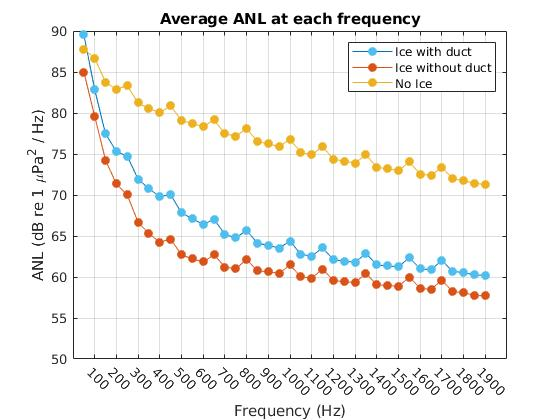
\includegraphics[scale=0.6]{Figures/Average_ANL.jpg}
\caption{Average ANL at frequencies from 50 to 1900 Hz.}
\label{fig_avg_anl}
\end{figure}

% CHANGE NAME ON FIGURE!!!
\begin{figure}[p]
\centering
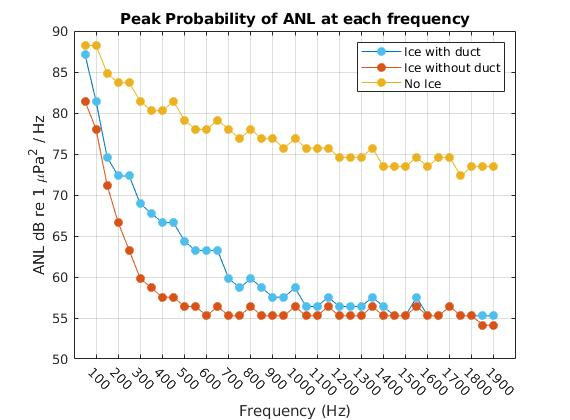
\includegraphics[scale=0.6]{Figures/peak_prob_ANL.jpg}
\caption{Peak probability or highest occurring bin value of ANL for frequencies from 50 to 1900 Hz.}
\label{fig_peak_prob}
\end{figure}

%%%%%%%%%%%%%%%%%%%%%%%%%%%%%%%%%%%%%%%%%%%%%%%%%%%%%%%%%%%%%%%%%%%%%55
\subsection{ANL Peak Probability} \label{sec_peak_prob}

Another single metric for describing the general nature of ANL under an environmental condition at each frequency is the peak probability, i.e. the most likely ANL value under that environment. As opposed to the average, this statistic metric leans heavily into the skew of the histogram. Looking at the peak probability may be better for describing the general trends of each acoustic environment's frequency. When compared, \autoref{fig_avg_anl} and \autoref{fig_peak_prob} display different changes in ANL and frequency. Peak probabilities were calculated using the following equation:

\begin{equation}
P(\mathcal{A},\omega)= \arg \max_{\omega} (\mathcal{H}_{i} [ANL ^{A}(\omega)]) 	% this is not actual stat distance 
\end{equation}
% argmax of hist-argmaxofhist, repeat equation

where $\mathcal{A}$ refers to the acoustic environment, $\mathcal{H}_{i}$ refers to the $i^{th}$histogram bin, $ANL^{\mathcal{A}}$ is the ambient noise at an environmental condition $A$, and $\omega$ is the frequency of interest.

%define eq here

% what is going on in peak probability
The yellow points denoting the peak probability for 'no ice' are highest, beginning at  90 dB and tapering down to approximately 75 dB. The curve of the 'no ice' line is the least steep. The blue points representing the peak probabilities of 'ice with duct' begin around 87 dB, close to 'no ice'. A steep drop in blue occurs from 100-700 Hz, and plateau at 57 dB. The red points of of 'ice without duct' behave similarly to the blue, but the decrease in ANL is more significant at lower frequency. 'Ice without duct' begins to plateau of 55 dB at 500 Hz.

For the lowest frequencies within \autoref{fig_peak_prob}, the difference between peaks is less than 10 dB, but the 'ice' conditions drop in ANL quickly. From 50-1000 Hz, the peak probabilities for 'ice with duct' remain between those of 'no ice' and 'ice without duct'. After this, overlap between the 'ice' conditions occurs. Similar to previous sections, 'no ice' is typically the loudest environmental condition, followed by 'ice with duct', then 'ice without duct'. \autoref{fig_peak_prob} does offer some key differences to this generalized pattern of sound level.

Unlike the averages in \autoref{fig_avg_anl} above, it appears that 'ice with duct' and 'ice without duct' share their most predominant ANL of 55 Hz. The separation of their averages is lost when peak probabilities are compared, suggesting that at frequencies above 1000 Hz, the Beaufort Duct is not as prevalent a factor. The peak probability line for 'no ice' is less steep than the average line for 'no ice', though the two run in the same general range. 

The peak probabilities are statistically the highest occurring sound level recorded by the SHRUs, and are therefore the most likely to occur under the environmental conditions presented in the future. In general, all the peak probability values for each frequency in \autoref{fig_peak_prob} are lower than those of the average values in \autoref{fig_avg_anl}. Comparing these peak probabilities numerically could show potential overall ambient noise level changes to the Arctic underwater noise environment.  


%%%%%%%%%%%%%%%%%%%%%%%%%%%%%%%%%%%%%%%%%%%%%%%%%%%%%%%%%%%%%%%%%%%%%%%%%%%%%%%%
\subsection{Pairwise Difference} \label{sec_pairdiff}

Using peak probabilities to generalize the ANL for each frequency above 1000 Hz, the ANL for 'ice with duct' and 'ice without duct' are almost the same. Comparing the differences between these peak probabilities is a reasonable method for finding a significant metric of the change between conditions. The metric used to make such a comparison is the pairwise difference between these probability distributions. Pairwise difference is the length between two bins at the same frequency between the two environmental noise types being analyzed. 

This metric is not measure of a probability but directly compares two decibel values between two environmental conditions. Pairwise difference in the context of this analysis represents the difference between the tallest noise level bar of each environmental condition, not the highest level of noise recorded. The pairwise difference for this analysis was calculated using the following equation:

%pair_dist_duct_noduct(i)=edges_duct(ind_duct(i))-edges_no_duct(ind_no_duct(i))
\begin{equation}
PD(\mathcal{A},\mathcal{B},\omega)=\mid \arg \max_{\omega} (\mathcal{H}_{i} [ANL ^{A}(\omega)])- \arg\max_{\omega}(\mathcal{H}_{i} [ANL^{B}(\omega)])\ \mid 	% this is not actual stat distance 
\end{equation}
% argmax of hist-argmaxofhist, repeat equation

where $\mathcal{A/B}$ refer to the two acoustic environments being compared, $\mathcal{H}_{i}$ refers to the $i^{th}$histogram bin, $ANL^{\mathcal{A/B}}$ is the ambient noise at an environmental condition $\mathcal{A}$ or $\mathcal{B}$, and $\omega$ is the frequency of interest. The x-axis of \autoref{fig_pairwisedist} graph is frequency in Hz, while the y-axis is the difference in ANL. The three environmental conditions produce three coupling differences, marked by three new colors. \autoref{fig_pairwisedist} labels the environments being compared through $PD$ with colors that are mixes of the primary colors from \autoref{fig_avg_anl}. Purple is the difference between 'ice with duct' and 'ice without duct', green is the difference between 'ice with duct' and 'no ice', and orange is the difference between 'ice without duct' and 'no ice'

The conditions with the highest overall difference are 'no ice' and 'ice without duct'. This orange line could represent the typical difference between the ambient noise with and without ice prior to the introduction of the Beaufort Duct. It begins with a steep increase in dB from 50-500 Hz, reaching a top difference of 24 dB at 450 Hz. After, the difference between 'ice without duct' and 'no ice' begins to decrease slightly, hovering around a 20 dB difference from 500-1900 Hz.

The middle difference condition comparison is between 'ice with duct' and 'no ice', represented by a green line and points. The difference between 'ice with duct' and 'no ice' reaches a maximum of 19 dB at 900 Hz and settles around 18 dB until 1900. Above 1000 Hz, the $PD$ for the orange and green lines are very similar, suggesting that there isn't a strong difference between the 'ice with duct' and 'ice without duct' noise levels when compared with 'no ice'. This  similarity between 'ice' conditions is emphasised by the third $PD$ line.

The conditions with the lowest overall difference are 'ice with duct' and 'ice without duct', represented by purple. Starting with a 6 dB difference at 50 Hz, there is a small decrease before the $PD$ between 'ice with duct' and 'ice without duct' maxes out at 9 dB. Following this maxima, the decibel values steadily decline before going near zero from 1100 Hz on. For half of its points, the purple line is more than 15 dB below the other two line's differences.  

This graph shows that the conditions 'ice with duct' and 'ice without duct' are very similar, while the conditions 'ice without duct' and 'no ice' are most different in ANL. One of the most interesting aspects of \autoref{fig_pairwisedist} is the insight into the significant band of frequencies the Beaufort Duct seems to affect the most. From 200 Hz to 600 Hz, the highest $PD$ between these conditions occurs at an average of 8 dB. This significant band is again reflected in the most separation between the orange and green lines occurring from 200 Hz to 600 Hz. The ambient noise of an environment with the Beaufort Duct is higher in ANL than an environment without the Duct. However, the separation between 'ice with duct' and 'ice without duct' does not encompass all frequencies, demonstrated by the overlap between the orange and green lines as frequency increases above 1000 Hz.

%%%%%%%%%%%%%%%%%%%%%%%%%%%%%%%%%%%%%%%%%%%%%%%%%%%%%%%%%%%%%%%%%%%%%%%%%%%%%%
% figures of total vart dist and pairwise dist
\begin{figure}[p]
\centering
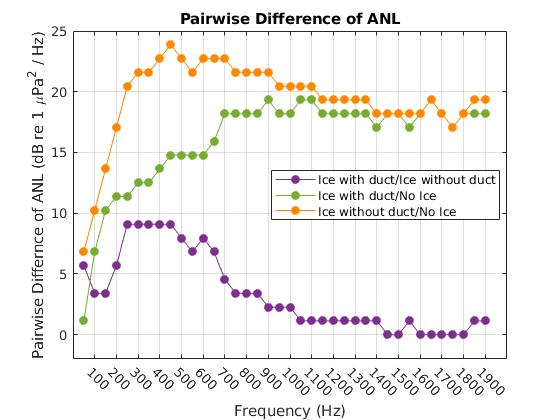
\includegraphics[scale=0.6]{Figures/recolor_pairwise_dist_ANLs2.jpg}
\caption{Pairwise distance for frequencies from 50 to 1900 Hz.}
\label{fig_pairwisedist}
\end{figure}

%% FIX LEGEND AGAIN
\begin{figure}[p]
\centering
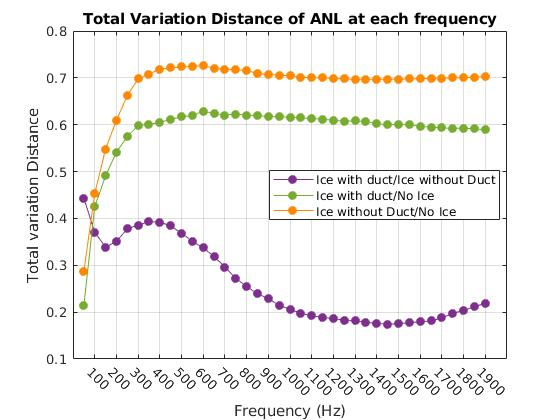
\includegraphics[scale=0.62]{Figures/recolor_total_var_dist_norm_pdf.jpg}
\caption{Total Variation distance for frequencies from 50 to 1900 Hz.}
\label{fig_totvardist}
\end{figure}

%%%%%%%%%%%%%%%%%%%%%%%%%%%%%%%%%%%%%%%%%%%%%%%%%%%%%%%%%%%%%%%%%%%%%%%%%%%%%%%%%%%
\subsection{Total Variation Distance} \label{sec_$TVD$}

Now, instead of point by point comparison, entire distributions will be compared. Rather than examine the statistic quantities of each acoustic environmental condition alone, one can compare the relationship between environments by frequency through total variation distance ($TVD$). This metric shows the likelihood between two probability distributions of acoustic environments. Unlike \autoref{sec_pairdiff}, this metric is a normalized value of probability, not a measure of sound level in decibels. Total variation distance essentially is the absolute area between two curves, showing how likely acoustic conditions will have overlap in their ANL distributions. 

 $TVD$ looks at all the data across all the frequencies, with the count of each bin as a proportion. It takes every value of the probability of that bin and takes the sum of the absolute difference between the two. This data set was normalized using PDF similar to the histograms in \autoref{sec_hist}. For the purposes of this analysis, the total variation distance uses the following equation: 

% equation used for our analysis
%\begin{equation} \label{eq:actualtotvar}
%\delta(Duct, No Duct)=\frac{1}{2} \Sigma \mid Duct(f) - No Duct(f) \mid 
%\end{equation}

\begin{equation} \label{tdv_eq}
    \delta_{ANL} ( \mathcal{A}, \mathcal{B}, \omega) = \frac{1}{2} \sum _{i} ^{} \mid \mathcal{H}_{i} [ANL^{\mathcal{A}}(\omega)] -\mathcal{H}_{i} [ANL^{\mathcal{B}}(\omega)] \mid 
\end{equation}

where  $\mathcal{H}_{i}$ is the \textit{i}th bin of the environmental condition histogram $\cal{H}$, $\omega$ is the frequency band, and $\cal{A/B}$ refer to the different environmental condition being compared. $\delta$ is the total variation difference between two ANL histograms of different environmental conditions. One number is returned by this equation that sums up the total variation distance between the two conditions. Values range from 0<$\delta$<1, where 1 means that two probability distributions are entirely different with no shared ANL values. An output value of 0 means the probability distribution are exactly the same, with the same occurrence of each ANL value, and intermediate values are intermediate situations.

\autoref{fig_totvardist} uses the same coloring convention as \autoref{fig_pairwisedist}, where purple is the difference between 'ice with duct' and 'ice without duct', green is the difference between 'ice with duct' and 'no ice', and orange is the difference between 'ice without duct' and 'no ice'. The x-axis are TVD values ranging from $0.1<\delta<0.8$ and the y-axis is frequency from 50-1900 Hz. The highest variation distance between the conditions ‘ice with duct' and 'ice without duct’ occurs at 50 Hz at $\delta$=0.44, between 'ice with duct' and 'No Ice' at 600 Hz and $\delta$=0.63, and between 'no ice' and 'ice without duct' at 600 Hz and $\delta$=0.72. There is always overlap between the three conditional pairs, though what dB values relate the two are not known. 

The highest $TVD$ line is the relationship between 'no ice' and 'no duct', represented by the orange points. Beginning at 0.3, the line increases from 50 Hz to 400 Hz and then plateaus at a value of 0.7. This indicates that the probability distributions for 'ice without duct' and 'no ice' do not have much in common. Looking at \autoref{fig_selhist} validates this, as the red and yellow bars of the respective histograms vary highly in shape. The middle green line represents the $TVD$ between 'ice with duct' and 'no ice'. Similar to the orange line, the green points rapidly increase from 50 Hz to 600 Hz, before plateauing around 0.6 for higher frequencies. This indicates that the probability distributions for 'ice with duct' and 'no ice' do have some overlap, but are still greater than 50\% different from each other. They are not as different as the conditions 'ice without duct' and 'no ice'. 

The lowest $TVD$ values belong to the conditions 'ice with duct' and 'ice without duct', showing that these two conditions are the most similar. The purple line begins below a value of 0.5, which is also the highest value achieved by this $TVD$. From 800 to 1900 Hz, it can be assumed that there is a significant amount of similarity in probability distributions between 'ice with duct' and 'ice without duct'. While purple shows the most similar between environments, a key aspect to this line is the bump from 50-1000 Hz where 'ice with duct' and 'ice without duct' are most different. LIke \autoref{fig_pairwisedist}, these bumps display where ANL(s) are higher for 'ice with duct.'

% The $TVD$ decrease to 0.35, before a slight increase from 150 Hz to 300 Hz to a $TVD$ of 0.4. Then the points decline under a $TVD$ of 0.2 until 1200 Hz, where there is another slight increase to above 0.2.

Similar to \autoref{fig_pairwisedist}, total variation distance shows that there is a significant band of frequencies where the difference between ambient noise with and without the Beaufort Duct is amplified. This is also corroborated by the green and orange line increasing in $TVD$ through a similar band of frequency. When the $TVD$ values for 'ice with duct' and 'ice without duct' are highest, the $TVD$ values for the green and orange points are lowest. Additionally, total variation distance as a whole is lower when the Duct is present when compared to an ice-free environment. This suggests that the sound makeup under these two environments is more similar than a traditionally duct-free area, likely attributed to ANL(s) with the Duct being closer in strength to an ice-free Arctic. As a whole, this displays that the Beaufort Duct makes the ambient soundscape louder.

%%%%%%%%%%%%%%%%%%%%%%%%%%%%%%%%%%%%%%%%%%%%%%%%%%%%%%%%%%%%%%%%%%%%%%%%%%%
% ADDITIONAL POSSIBLE SECTIONS?
% MAX, min, difference maxmin
% more histograms


%%%%%%%%%%%%%%%%%%%%%%%%%%%%%%%%%%%%%%%%%%%%%%%%%%%%%%%%%%%%%%%%%%%%%%%%%%%%%%
% can always add more like max min covariance more histograms, etc

% the end of statistic section
\section{Probability and Statistics Conclusions}
% a summary of the results from above 'the what it means' section
Using different methods of probability and statistics, certain generalizations about the soundscape of ambient noise in the Arctic can be made. The probability distributions of ambient noise show a 45 dB range of sound received between all three environmental conditions. As frequency increases, ANL decreases, with a minimum ambient noise around 55 dB. A clear difference between louder sound without ice and quieter sound with ice, regardless of Duct, exists as well. This decibel difference changes highly with frequency, something not seen before.

From this section, it is apparent that the Beaufort Duct has a strong effect on the level of noise under ice in the Arctic. The Duct's presence raises the ambient noise by up to 10 dB when compared to a ductless environment. However, this increase in noise is limited to a certain band of frequencies below 1000 Hz. It is unlikely that the Duct would cause the same ANL increase at higher frequencies. This results in similar noise levels above 1000 Hz, regardless of whether the Beaufort Duct is present or not.

